\documentclass{article}

\usepackage{fancyhdr} % Required for custom headers
\usepackage{lastpage} % Required to determine the last page for the footer
\usepackage{extramarks} % Required for headers and footers
\usepackage[usenames,dvipsnames]{color} % Required for custom colors
\usepackage{graphicx} % Required to insert images
\usepackage{listings} % Required for insertion of code
\usepackage{courier} % Required for the courier font
\usepackage{lipsum} % Used for inserting dummy 'Lorem ipsum' text into the template
\usepackage{amsmath}
\usepackage{amssymb}
\usepackage{mathtools, xparse}
\usepackage{booktabs}
\usepackage{bigstrut}
\usepackage{float}
\usepackage{hyperref}
\usepackage{color}
\usepackage{algorithm}
%\usepackage{caption}
\usepackage{algpseudocode}
\usepackage{multirow}
\usepackage{subfigure}
\usepackage{longtable}
\usepackage{supertabular}

\DeclarePairedDelimiter{\norm}{\lVert}{\rVert}
\DeclarePairedDelimiter\abs{\lvert}{\rvert}%

\hypersetup{
    colorlinks   = true,    % Colours links instead of ugly boxes
    urlcolor     = red,    % Colour for external hyperlinks
    linkcolor    = red,    % Colour of internal links
    citecolor    = red      % Colour of citations
}
% Margins
\topmargin=-0.45in
\evensidemargin=0in
\oddsidemargin=0in
\textwidth=6.5in
\textheight=9.0in
\headsep=0.25in

\linespread{1.1} % Line spacing

% Set up the header and footer
\pagestyle{fancy}
\lhead{\hmwkAuthorName} % Top left header
\chead{\hmwkClass\ : \hmwkID} % Top center head
\rhead{\firstxmark} % Top right header
\lfoot{\lastxmark} % Bottom left footer
\cfoot{} % Bottom center footer
\rfoot{Page\ \thepage\ of\ \protect\pageref*{LastPage}} % Bottom right footer
\renewcommand\headrulewidth{0.4pt} % Size of the header rule
\renewcommand\footrulewidth{0.4pt} % Size of the footer rule

\setlength\parindent{0pt} % Removes all indentation from paragraphs

%----------------------------------------------------------------------------------------
%	CODE INCLUSION CONFIGURATION
%----------------------------------------------------------------------------------------

\definecolor{MyDarkGreen}{rgb}{0.0,0.4,0.0} % This is the color used for comments
\lstloadlanguages{Perl} % Load Perl syntax for listings, for a list of other languages supported see: ftp://ftp.tex.ac.uk/tex-archive/macros/latex/contrib/listings/listings.pdf
\lstset{language=Perl, % Use Perl in this example
    frame=single, % Single frame around code
    basicstyle=\small\ttfamily, % Use small true type font
    keywordstyle=[1]\color{Blue}\bf, % Perl functions bold and blue
    keywordstyle=[2]\color{Purple}, % Perl function arguments purple
    keywordstyle=[3]\color{Blue}\underbar, % Custom functions underlined and blue
    identifierstyle=, % Nothing special about identifiers                                         
    commentstyle=\usefont{T1}{pcr}{m}{sl}\color{MyDarkGreen}\small, % Comments small dark green courier font
    stringstyle=\color{Purple}, % Strings are purple
    showstringspaces=false, % Don't put marks in string spaces
    tabsize=5, % 5 spaces per tab
    %
    % Put standard Perl functions not included in the default language here
    morekeywords={rand},
    %
    % Put Perl function parameters here
    morekeywords=[2]{on, off, interp},
    %
    % Put user defined functions here
    morekeywords=[3]{test},
    %
    morecomment=[l][\color{Blue}]{...}, % Line continuation (...) like blue comment
    numbers=left, % Line numbers on left
    firstnumber=1, % Line numbers start with line 1
    numberstyle=\tiny\color{Blue}, % Line numbers are blue and small
    stepnumber=5 % Line numbers go in steps of 5
}

% Creates a new command to include a perl script, the first parameter is the filename of the script (without .pl), the second parameter is the caption
\newcommand{\perlscript}[2]{
    \begin{itemize}
        \item[]\lstinputlisting[caption=#2,label=#1]{#1.py}
    \end{itemize}
}
\newcommand{\cppscript}[1]{
    \begin{itemize}
        \item[]\lstinputlisting[]{#1}
    \end{itemize}
}

%----------------------------------------------------------------------------------------
%	DOCUMENT STRUCTURE COMMANDS
%	Skip this unless you know what you're doing
%----------------------------------------------------------------------------------------

% Header and footer for when a page split occurs within a problem environment
\newcommand{\enterProblemHeader}[1]{
    \nobreak\extramarks{#1}{#1 continued on next page\ldots}\nobreak
    \nobreak\extramarks{#1 (continued)}{#1 continued on next page\ldots}\nobreak
}

% Header and footer for when a page split occurs between problem environments
\newcommand{\exitProblemHeader}[1]{
    \nobreak\extramarks{#1 (continued)}{#1 continued on next page\ldots}\nobreak
    \nobreak\extramarks{#1}{}\nobreak
}

%\setcounter{secnumdepth}{0} % Removes default section numbers
\newcounter{homeworkProblemCounter} % Creates a counter to keep track of the number of problems

\newcommand{\homeworkProblemName}{}
\newenvironment{homeworkProblem}[1][Problem \arabic{homeworkProblemCounter}]{ % Makes a new environment called homeworkProblem which takes 1 argument (custom name) but the default is "Problem #"
    \stepcounter{homeworkProblemCounter} % Increase counter for number of problems
    \renewcommand{\homeworkProblemName}{#1} % Assign \homeworkProblemName the name of the problem
    \section{\homeworkProblemName} % Make a section in the document with the custom problem count
    \enterProblemHeader{\homeworkProblemName} % Header and footer within the environment
    }{
    \exitProblemHeader{\homeworkProblemName} % Header and footer after the environment
}

\newcommand{\problemAnswer}[1]{ % Defines the problem answer command with the content as the only argument
\noindent\framebox[\columnwidth][c]{\begin{minipage}{0.98\columnwidth}#1\end{minipage}} % Makes the box around the problem answer and puts the content inside
}

\newcommand{\homeworkSectionName}{}
\newenvironment{homeworkSection}[1]{ % New environment for sections within homework problems, takes 1 argument - the name of the section
    \renewcommand{\homeworkSectionName}{#1} % Assign \homeworkSectionName to the name of the section from the environment argument
    \subsection{\homeworkSectionName} % Make a subsection with the custom name of the subsection
    \enterProblemHeader{\homeworkProblemName\ [\homeworkSectionName]} % Header and footer within the environment
    }{
    \enterProblemHeader{\homeworkProblemName} % Header and footer after the environment
}

%----------------------------------------------------------------------------------------
%	NAME AND CLASS SECTION
%----------------------------------------------------------------------------------------

\newcommand{\hmwkID}{homework 12} % Assignment title
\newcommand{\hmwkTitle}{RLC Circult}
\newcommand{\hmwkDueDate}{Tuesday,\ May\ 22,\ 2017} % Due date
\newcommand{\hmwkClass}{Numerical Analysis} % Course/class
\newcommand{\hmwkClassTime}{10:30am} % Class/lecture time
\newcommand{\hmwkClassInstructor}{Jones} % Teacher/lecturer
\newcommand{\hmwkAuthorName}{102061149 Fu-En Wang} % Your name

%----------------------------------------------------------------------------------------
%	TITLE PAGE
%----------------------------------------------------------------------------------------

\title{
    \vspace{2in}
    \textmd{\textbf{\hmwkClass}}\\
    \textmd{\textbf{\hmwkID: \hmwkTitle}} \\
    \normalsize\vspace{0.1in}\small{Due\ on\ \hmwkDueDate}\\
    \vspace{3in}
}

\author{\textbf{\hmwkAuthorName}}
\date{} % Insert date here if you want it to appear below your name

%----------------------------------------------------------------------------------------

\begin{document}
\maketitle
\newpage

\section{Introduction}
For a simple RLC circult as Figure \ref{fig:RLC}:
\begin{figure}[H]
    \centering
    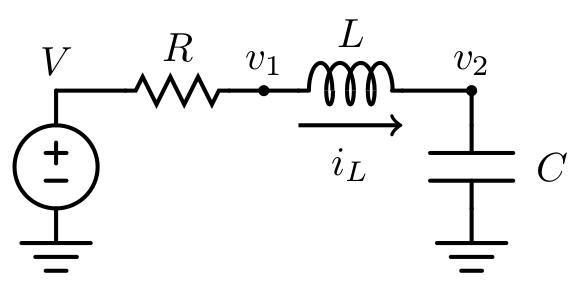
\includegraphics[width=0.4\textwidth]{src/RLC.jpg}
    \caption{RLC circult}
    \label{fig:RLC}
\end{figure}
The system consists of several ordinary differential equations:
\begin{align}
    & \frac{v_1 - V}{R} + i_L = 0 \\
    & \frac{dv_2}{dt} = \frac{i_L}{C} \\
    & \frac{di_L}{dt} = \frac{v_1 - v_2}{L}
\end{align}
In this homework, we will implement three algorithm to solve the ODE above.

\subsection{Forward Euler}
Forward Euler is to model ODE as 
$$
    x(t + h) = x(t) + h * f(t)
$$
and the system can be derived as
\begin{align}
    & v_1(t+h) = V + Ri_L(t+h) \\
    & v_2(t+h) = v_2(t) + \frac{h}{C}i_L(t) \\
    & i_L(t+h) = i_L(t) + \frac{h}{L}(v_1(t) - v_2(t))
\end{align}

\subsection{Backward Euler}
Backward Euler is to model ODE as
$$
    x(t + h) = x(t) + h * f(t+h)
$$
and the system can be derived as
\begin{align}
    & v_1(t+h) = V + Ri_L(t+h) \\
    & v_2(t+h) = v_2(t) + \frac{h}{C}i_L(t+h) \\
    & i_L(t+h) = i_L(t) + \frac{h}{L}(v_1(t+h) - v_2(t+h))
\end{align}
After some mathematical tricks, $i_L(t+h)$ can be derived as
\begin{align}
    i_L(t+h) = \frac{i_L(t) - \frac{h}{L}v_2(t) + \frac{hV}{L}}{1 + \frac{h^2}{LC} + \frac{hR}{L}}
\end{align}

\subsection{Trapezoidal}
\label{sec:trap}
Trapezoidal is to model ODE as 
$$
    x(t + h) = x(t) + h * \frac{f(t+h) + f(t)}{2}
$$
and the system can be derived as
\begin{align}
    & v_1(t+h) = V + R\frac{i_L(t+h) + i_L(t)}{2} \\
    & v_2(t+h) = v_2(t) + \frac{h}{2C}(i_L(t+h) + i_L(t)) \\
    & i_L(t+h) = i_L(t) + \frac{h}{2L}(v_1(t+h) - v_2(t+h) + v_1(t) - v_2(t))
\end{align}
After some mathematical tricks, $i_L(t+h)$ can be derived as
\begin{align}
    i_L(t+h) = \frac{(1-\frac{h^2}{4LC})i_L(t) + \frac{h}{2L}(V + v_1(t) - 2v_2(t))}{1 + \frac{h^2}{4LC} + \frac{hR}{2L}}
\end{align}

\section{Implementation}
\begin{algorithm}[H]
    \caption{\textbf{Ordinary Differential Equation}}
    \begin{algorithmic}
        \State t = start
        \While{t $<$ end\_time}
            \State Compute $x(t+h)$
            \State t += h
        \EndWhile
    \end{algorithmic}
\end{algorithm}

\section{Discussion}
In this section, we will discuss the result for different h and algorithm.

\subsection{Forward Euler}
When h = 0.1, Figure \ref{fig:for 01} shows v1, v2 and $i_L$ for $h \leq t \leq 10$
\begin{figure}[H]
    \centering
    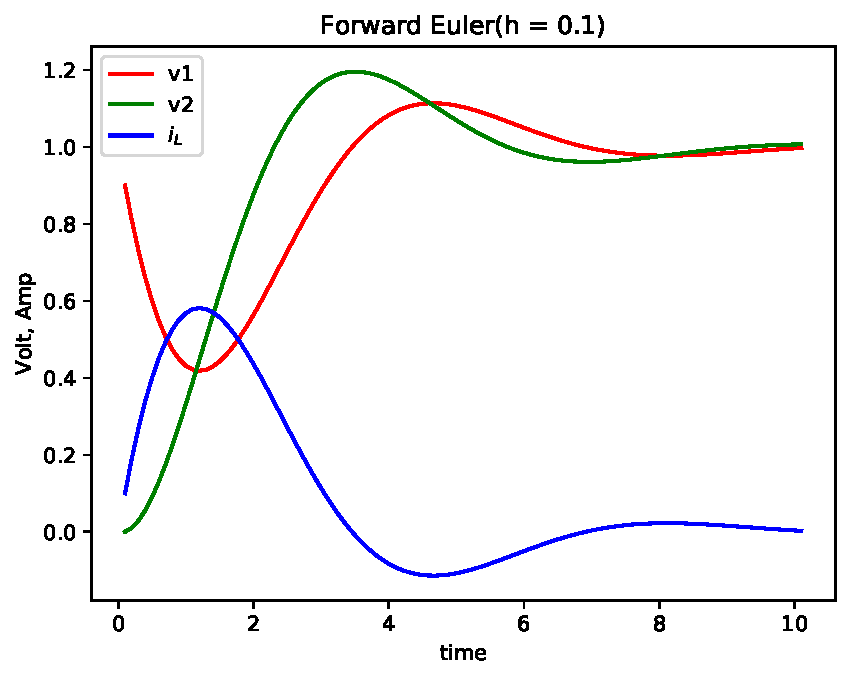
\includegraphics[width=0.6\textwidth]{src/for_01.pdf}
    \caption{Forward Euler(h = 0.1)}
    \label{fig:for 01}
\end{figure}
For the maximum and minimum value oof v1, v2 and $i_L$, Table \ref{tab:for 01} shows the result.
\begin{table}[H]
    \begin{center}
        \begin{tabular}{|c|c|c|c|}
            \hline
            Forward & V1 & V2 & iL \\ \hline
            Max & 1.1139 & 1.19627 & 0.581654 \\ \hline
            Min & 0.418346 & 0 & -0.113905 \\ \hline
        \end{tabular}
    \end{center}
    \caption{Max/Min of Forward Euler(h = 0.1)}
    \label{tab:for 01}
\end{table}

When h = 0.01, Figure \ref{fig:for 001} shows v1, v2 and $i_L$ for $h \leq t \leq 10$
\begin{figure}[H]
    \centering
    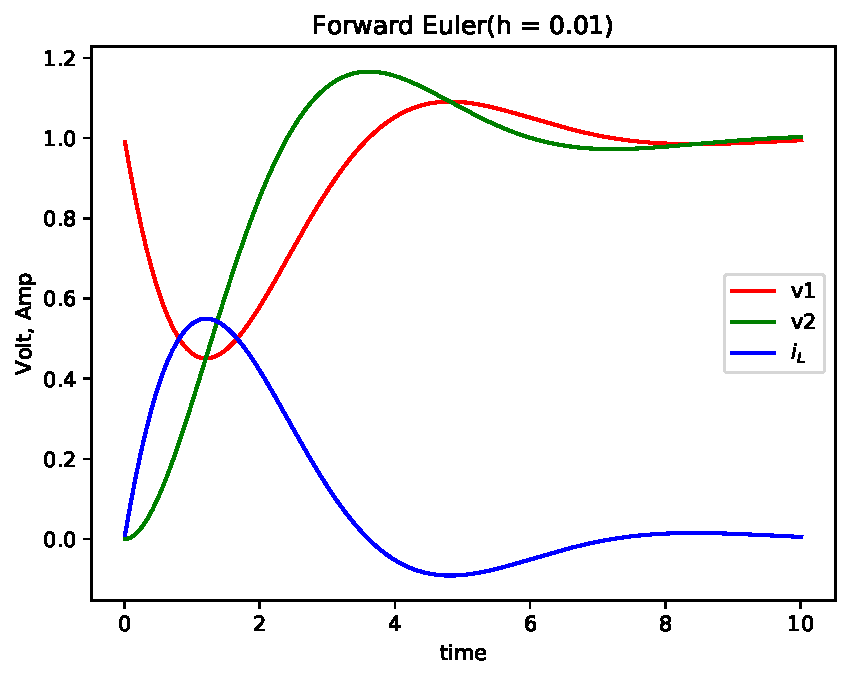
\includegraphics[width=0.6\textwidth]{src/for_001.pdf}
    \caption{Forward Euler(h = 0.01)}
    \label{fig:for 001}
\end{figure}
For the maximum and minimum value oof v1, v2 and $i_L$, Table \ref{tab:for 001} shows the result.
\begin{table}[H]
    \begin{center}
        \begin{tabular}{|c|c|c|c|}
            \hline
            Forward & V1 & V2 & iL \\ \hline
            Max & 1.09125 & 1.16602 & 0.549617 \\ \hline
            Min & 0.450383 & 0 & -0.0912488 \\ \hline
        \end{tabular}
    \end{center}
    \caption{Max/Min of Forward Euler(h = 0.01)}
    \label{tab:for 001}
\end{table}

\subsection{Backward Euler}
When h = 0.1, Figure \ref{fig:back 01} shows v1, v2 and $i_L$ for $h \leq t \leq 10$
\begin{figure}[H]
    \centering
    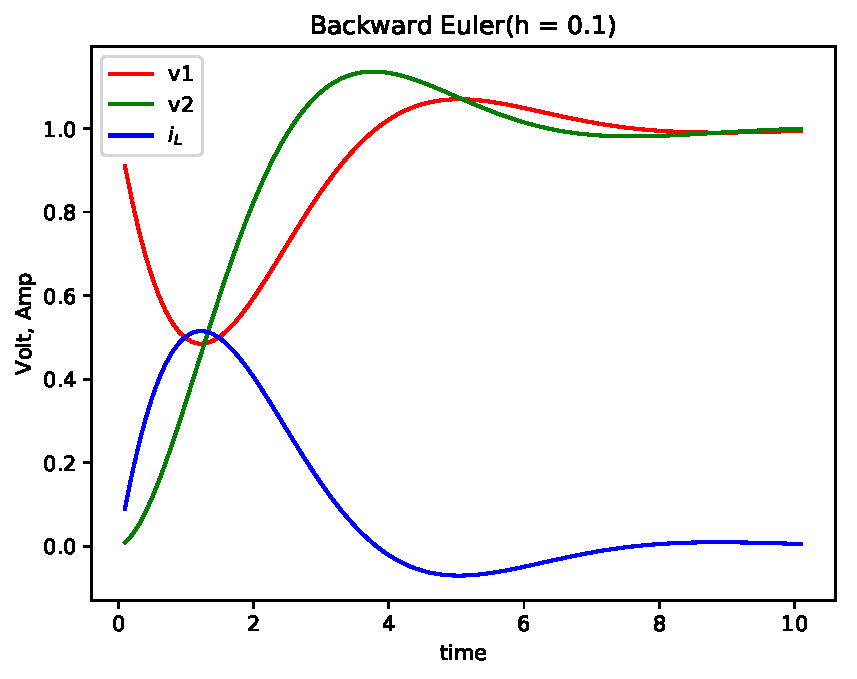
\includegraphics[width=0.6\textwidth]{src/back_01.pdf}
    \caption{Backward Euler(h = 0.1)}
    \label{fig:back 01}
\end{figure}
For the maximum and minimum value oof v1, v2 and $i_L$, Table \ref{tab:back 01} shows the result.
\begin{table}[H]
    \begin{center}
        \begin{tabular}{|c|c|c|c|}
            \hline
            Backward & V1 & V2 & iL \\ \hline
            Max & 1.07026 & 1.13651 & 0.515275 \\ \hline
            Min & 0.484725 & 0 & -0.0702564 \\ \hline
        \end{tabular}
    \end{center}
    \caption{Max/Min of Backward Euler(h = 0.1)}
    \label{tab:back 01}
\end{table}

When h = 0.01, Figure \ref{fig:back 001} shows v1, v2 and $i_L$ for $h \leq t \leq 10$
\begin{figure}[H]
    \centering
    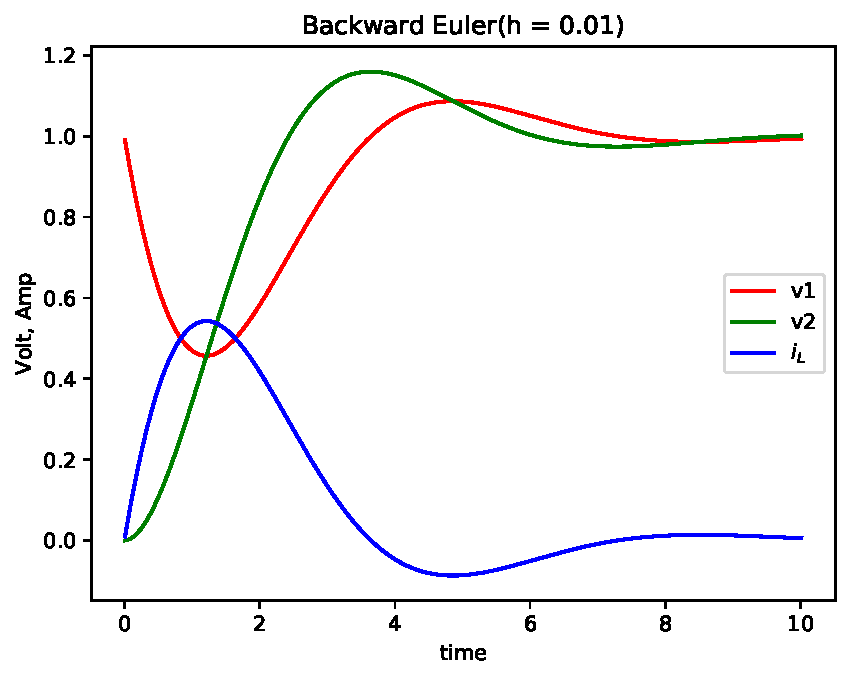
\includegraphics[width=0.6\textwidth]{src/back_001.pdf}
    \caption{Backward Euler(h = 0.01)}
    \label{fig:back 001}
\end{figure}
For the maximum and minimum value oof v1, v2 and $i_L$, Table \ref{tab:back 001} shows the result.
\begin{table}[H]
    \begin{center}
        \begin{tabular}{|c|c|c|c|}
            \hline
            Backward & V1 & V2 & iL \\ \hline
            Max & 1.08694 & 1.16011 & 0.543012 \\ \hline
            Min & 0.456988 & 0 & -0.0869399 \\ \hline
        \end{tabular}
    \end{center}
    \caption{Max/Min of Backward Euler(h = 0.01)}
    \label{tab:back 001}
\end{table}

\subsection{Trapezoidal}
When h = 0.1, Figure \ref{fig:trap 01} shows v1, v2 and $i_L$ for $h \leq t \leq 10$
\begin{figure}[H]
    \centering
    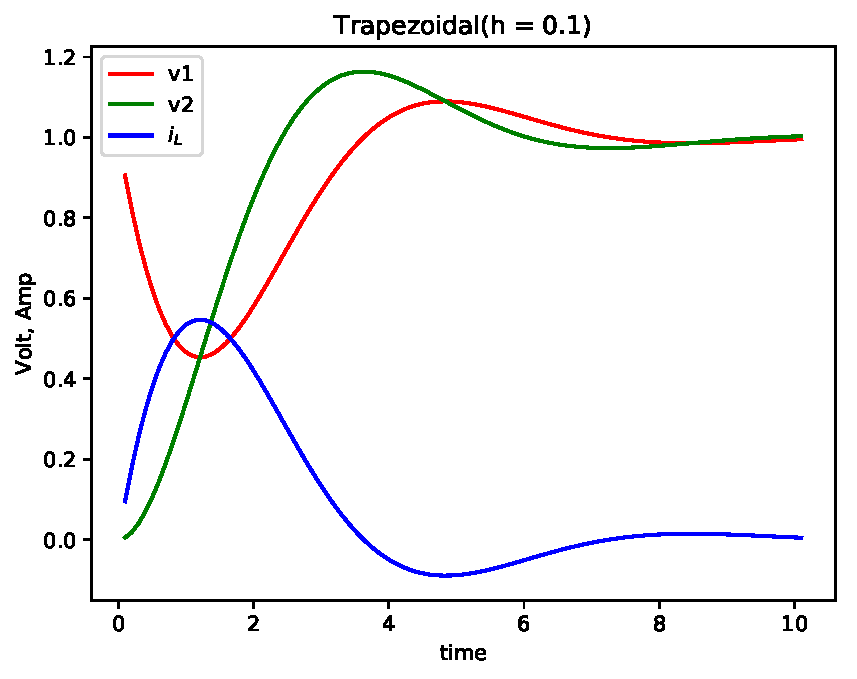
\includegraphics[width=0.6\textwidth]{src/trap_01.pdf}
    \caption{Trapezoidal(h = 0.1)}
    \label{fig:trap 01}
\end{figure}
For the maximum and minimum value oof v1, v2 and $i_L$, Table \ref{tab:trap 01} shows the result.
\begin{table}[H]
    \begin{center}
        \begin{tabular}{|c|c|c|c|}
            \hline
            Trap & V1 & V2 & iL \\ \hline
            Max & 1.08936 & 1.16346 & 0.546816 \\ \hline
            Min & 0.453184 & 0 & -0.0893592 \\ \hline
        \end{tabular}
    \end{center}
    \caption{Max/Min of Trapezoidal(h = 0.1)}
    \label{tab:trap 01}
\end{table}

When h = 0.01, Figure \ref{fig:trap 001} shows v1, v2 and $i_L$ for $h \leq t \leq 10$
\begin{figure}[H]
    \centering
    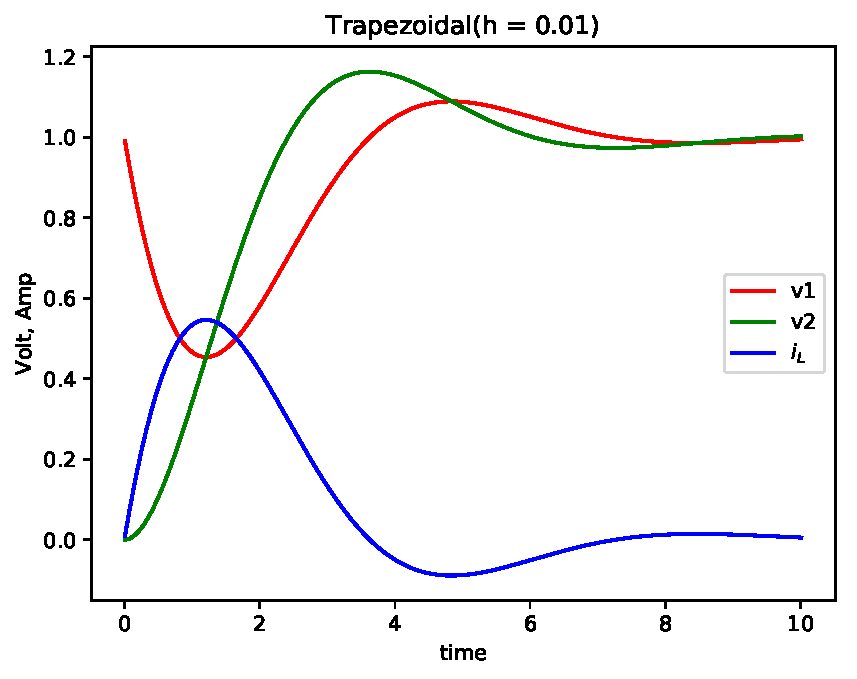
\includegraphics[width=0.6\textwidth]{src/trap_001.pdf}
    \caption{Trapezoidal(h = 0.01)}
    \label{fig:trap 001}
\end{figure}
For the maximum and minimum value oof v1, v2 and $i_L$, Table \ref{tab:trap 001} shows the result.
\begin{table}[H]
    \begin{center}
        \begin{tabular}{|c|c|c|c|}
            \hline
            Trap & V1 & V2 & iL \\ \hline
            Max & 1.08907 & 1.16304 & 0.546298 \\ \hline
            Min & 0.453702 & 0 & -0.0890672 \\ \hline
        \end{tabular}
    \end{center}
    \caption{Max/Min of Trapezoidal(h = 0.01)}
    \label{tab:trap 001}
\end{table}

\subsection{Comparison}
For convenient purpose, I merge the four tables above as Table \ref{tab:all 01} and \ref{tab:all 001}
\begin{table}[H]
    \begin{center}
        \begin{tabular}{|c|c|c|c|}
            \hline
            Forward & V1 & V2 & iL \\ \hline
            Max & 1.1139 & 1.19627 & 0.581654 \\ \hline
            Min & 0.418346 & 0 & -0.113905 \\ \hline
              &  &  &  \\ \hline
              Backward & V1 & V2 & iL \\ \hline
              Max & 1.07026 & 1.13651 & 0.515275 \\ \hline
              Min & 0.484725 & 0 & -0.0702564 \\ \hline
               &  &  &  \\ \hline
               Trap & V1 & V2 & iL \\ \hline
               Max & 1.08936 & 1.16346 & 0.546816 \\ \hline
               Min & 0.453184 & 0 & -0.0893592 \\ \hline
        \end{tabular}
    \end{center}
    \caption{Max/Min(h = 0.1)}
    \label{tab:all 01}
\end{table}
\begin{table}[H]
    \begin{center}
        \begin{tabular}{|c|c|c|c|}
            \hline
            Forward & V1 & V2 & iL \\ \hline
            Max & 1.09125 & 1.16602 & 0.549617 \\ \hline
            Min & 0.450383 & 0 & -0.0912488 \\ \hline
              &  &  &  \\ \hline
              Backward & V1 & V2 & iL \\ \hline
              Max & 1.08694 & 1.16011 & 0.543012 \\ \hline
              Min & 0.456988 & 0 & -0.0869399 \\ \hline
               &  &  &  \\ \hline
               Trap & V1 & V2 & iL \\ \hline
               Max & 1.08907 & 1.16304 & 0.546298 \\ \hline
               Min & 0.453702 & 0 & -0.0890672 \\ \hline
        \end{tabular}
    \end{center}
    \caption{Max/Min(h = 0.01)}
    \label{tab:all 001}
\end{table}
From the two tables, we can find that the value of Trapezoidal is between that of Forward and Backward Euler. Recall from Section \ref{sec:trap},
the formula of Trapezoidal is:
$$
    x(t+h) = x(t) + h * \frac{f(t+h) + f(t)}{2}
$$
The part $\frac{f(t+h) + f(t)}{2}$ is the mean value of that of Forward and Backward. As a result, it seems reasonable we got a value between the 
two method.


\end{document}













